%\VignetteIndexEntry{Answer 06 from Seminar III: R/Bioconductor}
%\VignetteDepends{}
%\VignetteKeywords{R, Bioconductor}
%\VignettePackage{SIII: R/Bioc}
\documentclass[letterpaper,12pt]{article}

%%%%%%%%%%%%%%%%%%%%%%%% Standard Packages %%%%%%%%%%%%%%%%%%%%%%%%%%%%%%%%%%%%%%%%%%
%\usepackage{epsfig}
%\usepackage{graphicx}
%\usepackage{graphics}
%\usepackage{amssymb}
%\usepackage{amsmath}
%\usepackage{mathrsfs}
%\usepackage{caption}
%\usepackage{comment}
\usepackage{fancyvrb}
\usepackage{fancyhdr}

\usepackage[a4paper]{geometry}
\usepackage{hyperref,graphicx}

%\usepackage[spanish]{babel}
%\selectlanguage{spanish}
%\usepackage[utf8]{inputenc}

%%%%%%%%%%%%%%%%%%%%%% some personal commands %%%%%%%%%%%%%%%%%%%%%%%%%%%%%%%%%%%%%%%%%%%%
\newcommand{\pl}[1]{\texttt{#1}}
\newcommand{\myurlshort}[2]{\href{http://#1}{{\textsf{#2}}}}

%%%%%%%%%%%%%%%%%%%%%% headers and footers %%%%%%%%%%%%%%%%%%%%%%%%%%%%%%%%%%%%%%%%%%%%
\pagestyle{fancy} 
\renewcommand{\footrulewidth}{\headrulewidth}

%%%%%%%%%%%%%%%%%%%%%%%%% bibliography  %%%%%%%%%%%%%%%%%%%%%%%%%%%%%%%%%%%%%%%%%%%%%%%
\bibliographystyle{plainnat}

%%%%%%%%%%%%%%%%%%%%%%%%% sweave options  %%%%%%%%%%%%%%%%%%%%%%%%%%%%%%%%%%%%%%%%%%%%%%%




%%%%%%%%%%%%%%%%%%%%%%% opening %%%%%%%%%%%%%%%%%%%%%%%%%%%%%%%%%%%%
\title{\textbf{Seminar III: \texttt{R}/\texttt{Bioconductor}\\ \small August-December 2009}}
\author{Leonardo Collado Torres\\[1em]Bachelor in Genomic Sciences (LCG),\\ UNAM, Cuernavaca, Mexico\\[1em]\texttt{lcollado@lcg.unam.mx}\\[1em]\url{http://www.lcg.unam.mx/~lcollado/}}

\usepackage{Sweave}
\begin{document}
\maketitle

\medskip
\noindent{\small\textbf{Assistants:} Alejandro Reyes \pl{areyes@lcg.unam.mx}, Jos\'e Reyes \pl{jreyes@lcg.unam.mx} and V\'ictor Moreno \pl{jmoreno@lcg.unam.mx}}

\medskip
\noindent{\small\textbf{Note:} Questions through the \myurlshort{foros.nnb.unam.mx/viewforum.php?f=111}{forum} please. Those who are not from the sixth LCG generation send us an email so we can register you on the forum.}

\medskip
\begin{abstract}
The following exercise will make sure that you can use the \pl{GenomeGraphs} package.
\end{abstract}

\section{GenomeGraphs}
  \begin{enumerate}
  \item Download the following paper by Durinck, Bullard, Spellman and Dudoit: \url{http://www.ncbi.nlm.nih.gov/pubmed/19123956}
  \item Reproduce figure 3 from the paper. Its just a matter of extracting the code from the text :) \scriptsize
\begin{Schunk}
\begin{Sinput}
> library(GenomeGraphs)
> data("seqDataEx", package = "GenomeGraphs")
> str = seqDataEx$david[, "strand"] == 1
> biomart = useMart("ensembl", "scerevisiae_gene_ensembl")
> a <- makeGeneRegion(chromosome = "IV", start = 1300000, end = 1310000, 
+     strand = "-", biomart = biomart, dp = DisplayPars(plotId = TRUE, 
+         idRotation = 0, cex = 0.5))
> b <- makeGenomeAxis(dp = DisplayPars(byValue = 1000, size = 3))
> c <- makeGeneRegion(chromosome = "IV", start = 1300000, end = 1310000, 
+     strand = "+", biomart = biomart, dp = DisplayPars(plotId = TRUE, 
+         idRotation = 0, cex = 0.5))
> d <- makeBaseTrack(base = seqDataEx$snyder[, "location"], value = seqDataEx$snyder[, 
+     "counts"], dp = DisplayPars(lwd = 0.3, color = "darkblue", 
+     ylim = c(0, 300)))
> e <- makeGenericArray(probeStart = seqDataEx$david[str, "location"], 
+     intensity = seqDataEx$david[str, "expr", drop = FALSE], dp = DisplayPars(pointSize = 0.5))
> f <- makeGenericArray(probeStart = seqDataEx$david[!str, "location"], 
+     intensity = seqDataEx$david[!str, "expr", drop = FALSE], 
+     dp = DisplayPars(color = "darkgreen", pointSize = 0.5))
> g <- makeBaseTrack(base = seqDataEx$nislow[, "location"], value = seqDataEx$nislow[, 
+     "evalue"], dp = DisplayPars(color = "grey", lwd = 0.25))
> h <- makeBaseTrack(base = seqDataEx$conservation[, "location"], 
+     value = seqDataEx$conservation[, "score"], dp = DisplayPars(color = "gold4", 
+         lwd = 0.25))
> pList <- list(`-` = a, b, `+` = c, Nagalakshmi = d, `David +` = e, 
+     `David -` = f, Lee = g, Conservation = h)
> rOverlay <- makeRectangleOverlay(start = 1302105, end = 1302190, 
+     region = c(4, 8), dp = DisplayPars(alpha = 0.2))
> gdPlot(pList, minBase = 1301500, maxBase = 1302500, overlay = rOverlay)
\end{Sinput}
\end{Schunk}
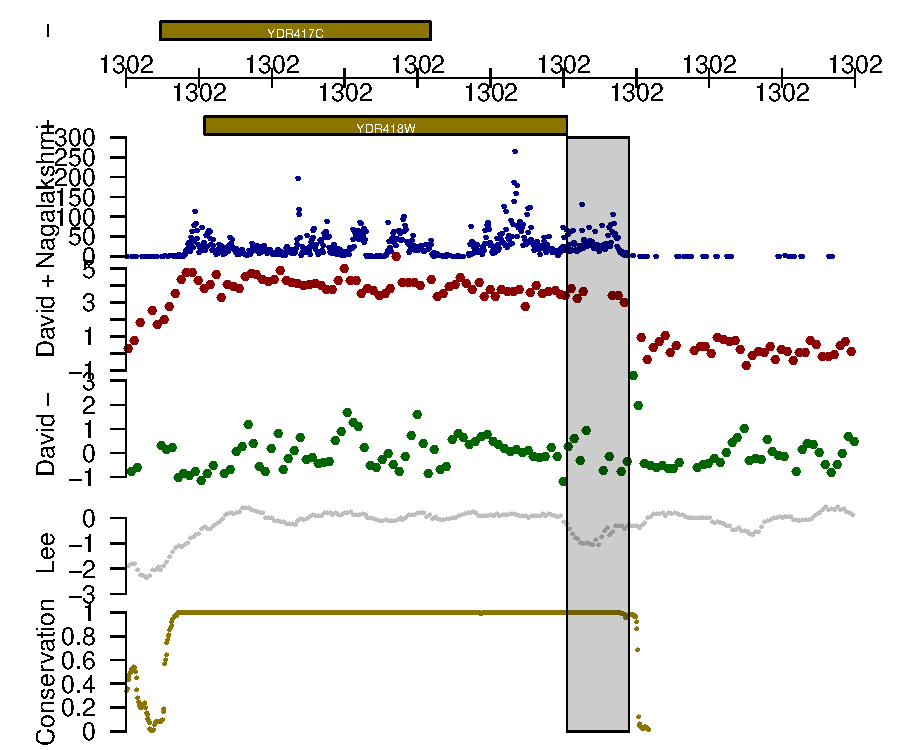
\includegraphics{plots/fig-001}
  \item \normalsize Make a new plot with some re-ordering: invert the order of tracks. Meaning that you'll have conservation on top, followed by the Lee data, then David -, David +, Nagalakshmi, + gene region, genome axis, and finally - gene region. Change the colors of all the tracks to any ones you like (without repeating them). Finally, add a text overlay with your username on the conservation track around positions 1301700 to 1301900. You might prefer to build each \pl{gdObject} like in the class (a, b, c, \ldots) and then create the list when you use \pl{gdPlot}. \scriptsize
\begin{Schunk}
\begin{Sinput}
> a <- makeGeneRegion(chromosome = "IV", start = 1300000, end = 1310000, 
+     strand = "-", biomart = biomart, dp = DisplayPars(protein_coding = "darkblue", 
+         plotId = TRUE, idRotation = 0, cex = 0.5))
> b <- makeGenomeAxis(dp = DisplayPars(byValue = 1000, size = 3))
> c <- makeGeneRegion(chromosome = "IV", start = 1300000, end = 1310000, 
+     strand = "+", biomart = biomart, dp = DisplayPars(protein_coding = "darkblue", 
+         plotId = TRUE, idRotation = 0, cex = 0.5))
> d <- makeBaseTrack(base = seqDataEx$snyder[, "location"], value = seqDataEx$snyder[, 
+     "counts"], dp = DisplayPars(lwd = 0.3, color = "yellow", 
+     ylim = c(0, 300)))
> e <- makeGenericArray(probeStart = seqDataEx$david[str, "location"], 
+     intensity = seqDataEx$david[str, "expr", drop = FALSE], dp = DisplayPars(color = "purple", 
+         pointSize = 0.5))
> f <- makeGenericArray(probeStart = seqDataEx$david[!str, "location"], 
+     intensity = seqDataEx$david[!str, "expr", drop = FALSE], 
+     dp = DisplayPars(color = "green", pointSize = 0.5))
> g <- makeBaseTrack(base = seqDataEx$nislow[, "location"], value = seqDataEx$nislow[, 
+     "evalue"], dp = DisplayPars(color = "blue", lwd = 0.25))
> h <- makeBaseTrack(base = seqDataEx$conservation[, "location"], 
+     value = seqDataEx$conservation[, "score"], dp = DisplayPars(color = "red", 
+         lwd = 0.25))
> pList <- list(Conservation = h, Lee = g, `David -` = f, `David +` = e, 
+     Nagalakshmi = d, `+` = c, b, `-` = a)
> rOverlay <- makeRectangleOverlay(start = 1302105, end = 1302190, 
+     region = c(1, 5), dp = DisplayPars(alpha = 0.2))
> tOverlay <- makeTextOverlay("lcollado", 1301900, 0.5, region = c(1, 
+     1), dp = DisplayPars(color = "black"))
> gdPlot(pList, minBase = 1301500, maxBase = 1302500, overlays = c(rOverlay, 
+     tOverlay))
\end{Sinput}
\end{Schunk}
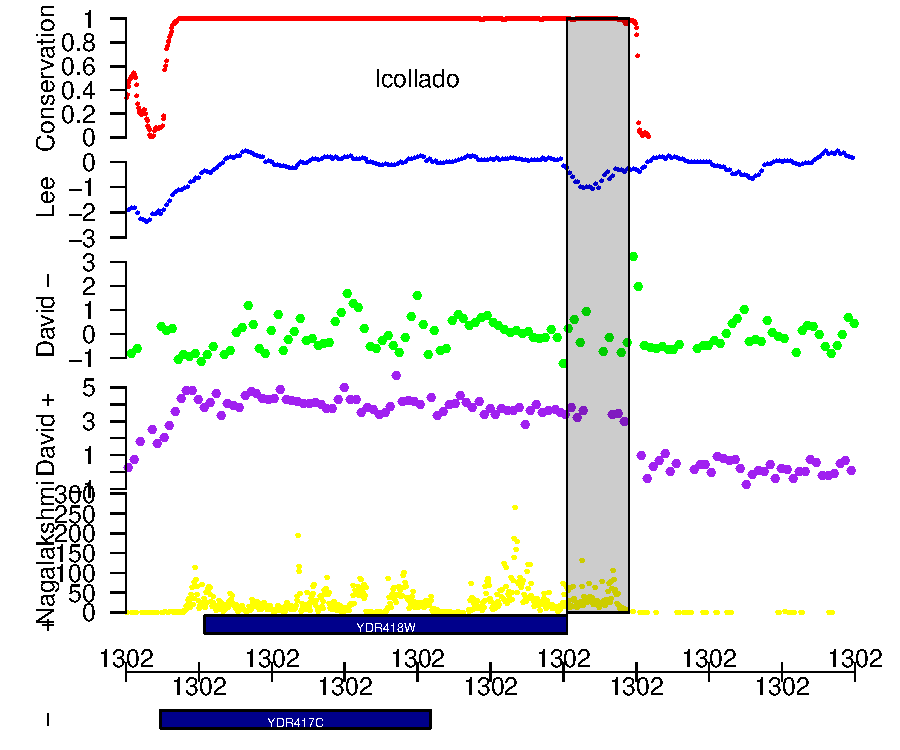
\includegraphics{plots/fig-002}
  \item \normalsize Explain every "make\ldots" command :)
  \begin{itemize}
  \item To create object \pl{a} I used \pl{makeGeneRegion} which uses biomaRt to find the protein coding genes on the negative strand on yeast chromosome IV from bases 1300000 to 1310000. It adds the names in white and makes dark blue boxes for the protein coding regions.
  \item To create object \pl{b} I used \pl{makeGenomeAxis} which simply creates the genome axis with a tick every 1000 base pairs.
  \item Object \pl{c} is very similar to object \pl{a} except that it looks for protein coding regions on the plus strand.
  \item Object \pl{d} uses the snyder data frame (Nagalakshmi data) and plots the points in yellow. The points plotted are those within 0 and 300.
  \item Object \pl{e} plots the data for the plus strand using the david data frame. The points are in purple with a smaller point size. As this in array data, I used \pl{makeGenericArray}.
  \item Object \pl{f} is very similar to object \pl{e} except that it plots the points in green and it uses the data for the negative strand.
  \item Object \pl{g} plots the Lee data in blue using the nislow data frame.
  \item Object \pl{h} plots in red the conservation information using the data frame with the same name.
  \item \pl{rOverlay} and \pl{tOverlay} are rectangle and text overlays. The rectangle one covers tracks 1 to 5 and helps highlight a region of interest. I used the text overlay to add my username to the plot.
  \end{itemize}
  \end{enumerate}


\end{document}
